\begin{figure}[ht]
\centering
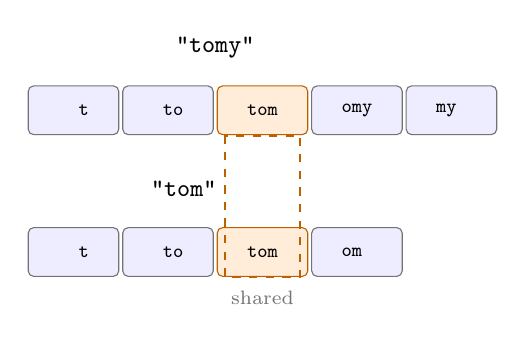
\begin{tikzpicture}[font=\small,
  tg/.style={draw=black!55, fill=blue!7, rounded corners=2pt,
             minimum width=1.15cm, minimum height=0.62cm,
             inner sep=3pt, align=center, font=\scriptsize},
  sh/.style={draw=orange!75!black, fill=orange!15, rounded corners=2pt,
             minimum width=1.15cm, minimum height=0.62cm,
             inner sep=3pt, align=center, font=\scriptsize}
]
\node[font=\small\bfseries] at (1.8, 1.6) {\texttt{"tomy"}};
\node[tg] at (0.0,  0.8) {\texttt{\ \ t}};
\node[tg] at (1.2,  0.8) {\texttt{\ to}};
\node[sh] at (2.4,  0.8) {\texttt{tom}};
\node[tg] at (3.6,  0.8) {\texttt{omy}};
\node[tg] at (4.8,  0.8) {\texttt{my\ }};
\node[font=\small\bfseries] at (1.4, -0.2) {\texttt{"tom"}};
\node[tg] at (0.0, -1.0) {\texttt{\ \ t}};
\node[tg] at (1.2, -1.0) {\texttt{\ to}};
\node[sh] at (2.4, -1.0) {\texttt{tom}};
\node[tg] at (3.6, -1.0) {\texttt{om\ }};
\draw[draw=orange!75!black, thick, dashed] (1.92, 0.48) rectangle (2.88, -1.32);
\node[font=\scriptsize, black!55] at (2.4, -1.58) {shared};
\end{tikzpicture}
\caption{Trigram decomposition and shared-trigram similarity scoring.}
\end{figure}
